\documentclass[tikz]{standalone}

\usepackage{tikz}
\usetikzlibrary{calc}

\begin{document}

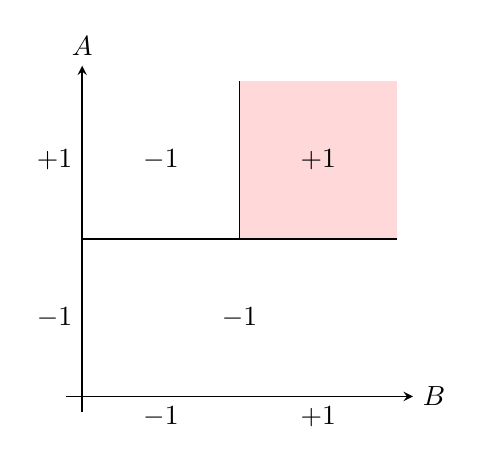
\begin{tikzpicture}[>=stealth,line width=0.5pt]
    \fill[red!15] (2,2) rectangle (4,4);
    % Axes
    \draw[->] (-0.2,0) -- (4.2,0) node[right] {$B$};
    \draw[->] (0,-0.2) -- (0,4.2) node[above] {$A$};

    % Horizontal and vertical split lines
    \draw (0,2) -- (4,2);
    \draw (2,2) -- (2,4);

    % Highlight the top-right cell (in light pink)
    

    % Region labels
    \node at (1,3) {$-1$};
    \node at (3,3) {$+1$};
    \node at (2,1) {$-1$};
    % \node at (3,1) {$-1$};

    % Axis tick labels (+1 / -1)
    \node[left] at (0,3) {$+1$};
    \node[left] at (0,1) {$-1$};

    \node[below] at (1,0) {$-1$};
    \node[below] at (3,0) {$+1$};

\end{tikzpicture}

\end{document}